% add --shell-escape to pdflatex arguments.
\documentclass[14pt]{extarticle}
\usepackage[left=2cm , right = 2cm, top=2cm]{geometry}
\usepackage{helvet}
\usepackage{parskip}
\usepackage{amsmath}
\usepackage{amssymb}
\usepackage{graphicx}
\usepackage[spanish]{babel}
\usepackage[dvipsnames]{xcolor}
\usepackage{tcolorbox} % above of the svg package
\usepackage{svg} 
\usepackage{hyperref}
\usepackage{minted}
\renewcommand{\sfdefault}{lmss}  % este activa la letra lmss
\renewcommand{\familydefault}{\sfdefault} % este activa la letra lmss
\sffamily % este activa la letra lmss
%\hyperlink{page.2}{Go to page 2}
%\newpage
%text on page 2
%\begin{figure}[htbp]
%  \centering
%  \includesvg{plot.svg}
%  \caption{svg image}
%\end{figure}

%\begin{minted}{csharp}
%    // single comment
%    \end{minted}

%\begin{align}
%    \frac{d}{dx} \ln x &= \lim_{h\to 0} \frac{\ln(x+h) - \ln x}{h} \\
%    &= \ln e^{1/x} &&\text{How this follows is left as an exercise.}\\
%    &= \frac{1}{x} &&\text{Using the definition of ln as inverse function}
%   \end{align}




\begin{document}



@BritoAlv @DavierSanBel
\tableofcontents
\section{Cómo funciona el algoritmo}
\subsection{Enunciado Particularizado}
\begin{tcolorbox}[colback=blue!5!white,colframe=blue!75!black, title = Insertion Sort]
Empecemsos con una versión \textbf{particularizada} de el problema: Dado un \textbf{array} de \textbf{int} ordenarlos de menor a mayor, usando el algoritmo de insertion sort. 
\end{tcolorbox}
\subsection{El algoritmo}

El algoritmo \textbf{recorre el array} desde la segunda posición ($i=1$) hasta la última $N$, garantizando que al pasar por la posición $i$, el arreglo que va desde $[0,i]$ está \textbf{sorted}, notemos que inicialmente para $i=0$ esto se cumple (porque es de longitud $1$), el algoritmo mantiene esto invariante a medida que se va ejecutando y esto es su base.
\begin{center}
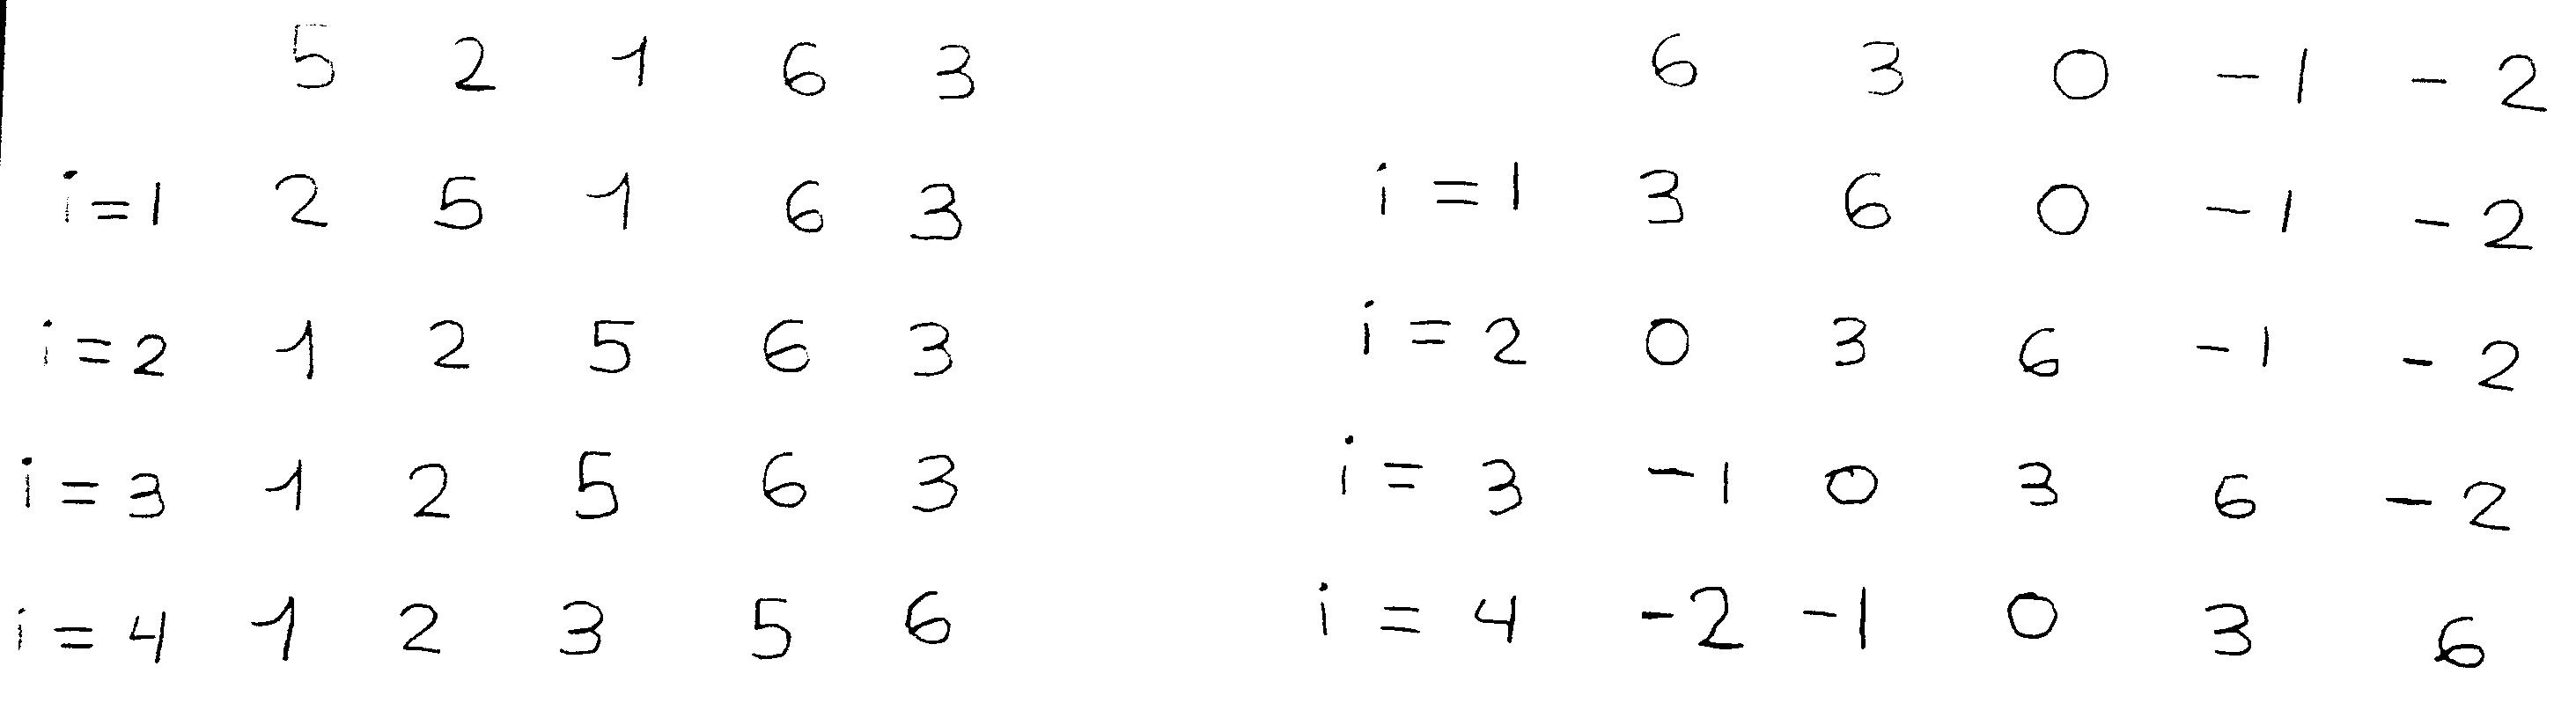
\includegraphics[width=18cm,height=17cm,keepaspectratio]{Fa}    
\end{center}


Existen dos formas de implementar el insertion sort. (¿qué ocurre dentro del for para \textbf{sort the array}?)

\begin{enumerate}
    \item Usando \textbf{swap}, un swap es intercambiar dos elementos consecutivos, por lo que si queremos hallar donde va el elemento $i$ en el subarreglo de $[0,i-1]$ comparamos y hacemos swap hasta llegar a la posición buscada.
% some picture indicating insertion sort using swaps.
    \item Usando \textbf{binary search} para hallar la posición $k$ donde se va a insertar y después shift los elementos a la derecha de $k$.
    
% some picture indicating insertion sort using binary search. 
  
\end{enumerate}
\begin{center}
    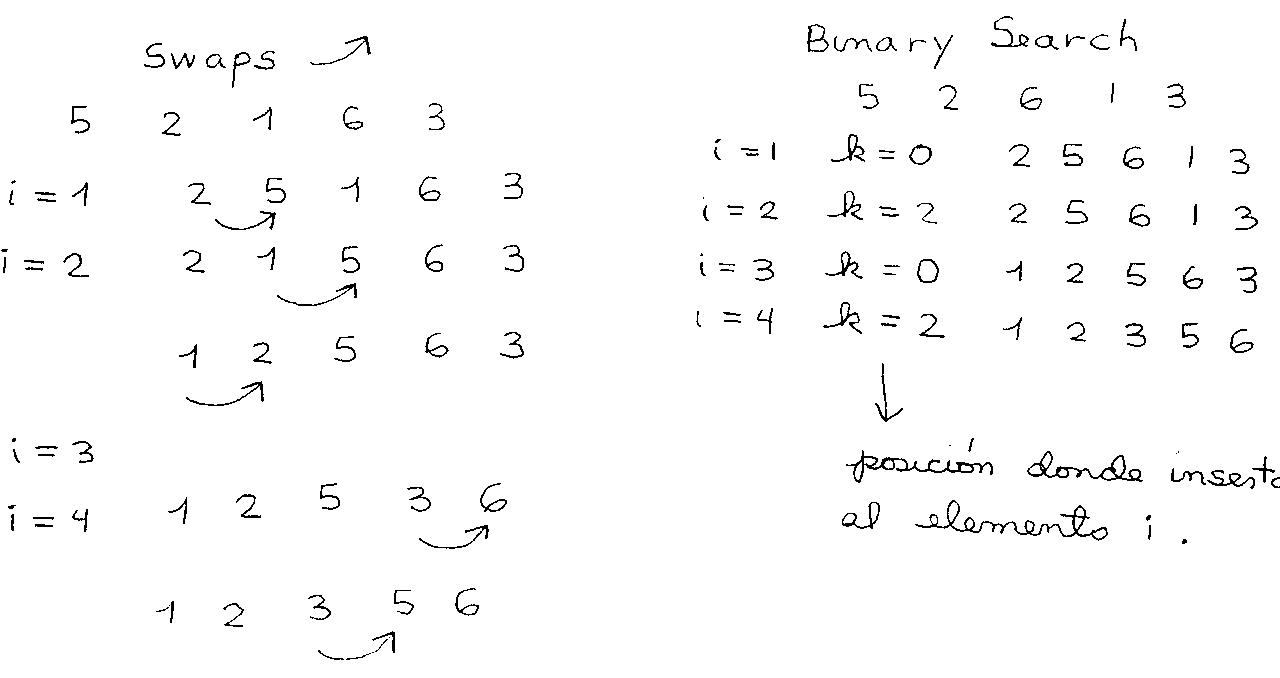
\includegraphics[width=20cm,height=10cm,keepaspectratio]{E}    
    \end{center} 
\section{Implementación}
\subsection{Usando Swaps}
\begin{minted}{csharp}
    public static void swaps_0(int[] source)
    /* 
    The thing is that inside the while there are three
    constant operations.
    */
    {
        for (int i = 1; i < source.Length; i++) // n-1 iterations, so O(n)
        {
            int j = i;
            // the array from position 0 to j-1 is sorted always,
            // so now insert source[i] in that array, keeping it sorted.
            while((j > 0) && (source[j-1] > source[j]) ) 
            // has to go from i-1 to 0, checking, in each check,
            // it compares and after that do the swap.
            {                
                int temp = source[j-1]; 
                source[j-1] = source[j];
                source[j] = temp;
                j--;
            }
        }
    }
\end{minted}

\subsection{Usando Binary Search}
\begin{minted}{csharp}

    public static void binary_search_0(int[] source)
    {
        for (int i = 1; i < source.Length; i++) // n-1 iterations, so O(n)
        {
            // the array from position 0 to j-1 is sorted always, so now 
            //insert source[i] in that array, keeping it sorted.
            // binary search to insert source[i] in correct position.
            // find index where to insert, and after that shift indexes.
            int l = 0;
            int r = i-1;
            int mid = 0;
            while(r-l > 1)
            // as long as l-r > 1 we ensure that l < r and that mid is
            // inside
            {
                mid = (l+r)/2;
                if( source[mid] == source[i])
                {
                    l = mid;
                    r = mid;
                }
                else if ( source[mid] > source[i])
                {
                    r = mid-1;
                }
                else
                {
                    l = mid+1;
                }
            }
            // we have either l = r or r = l+1 bases cases of recursivity.
            int pos;
            if (source[i] <= source[l])
            {
                pos = l; //
            }
            else if(source[i] > source[r] )
            {
                pos = r+1; // 
            }
            else
            {
                pos = r;
            }
            int temp = source[i];
            // shift process
            for (int j = i; j >= pos+1; j--)
            {
                source[j] = source[j-1];
            }
            source[pos] = temp;
        }        
    }    

\end{minted}

\section{Complejidad del Algoritmo}

Para calcular la complejidad del algoritmo, debemos calcular cuantas operaciones primitivas realiza en términos de $N$, usando los siguientes datos:

\begin{enumerate}
    \item Inicializar un objeto de tipo \textbf{int} es en tiempo constante.
    \item Random access en un array es en tiempo constante.
    \item Comparar dos enteros es en tiempo constante.
\end{enumerate}
 
\textbf{Nota 1:} El proceso de shift los elementos es linear respecto a la cantidad de elementos.

\subsection{Swaps}

Se inicializa $i$.  Veamos para cada iteración $i$ del \textbf{for} cuantas operaciones se realizan:

\begin{itemize}
    \item se inicializa $j$.
    \item La mayor cantidad de veces que puede ser ejecutado el \textbf{while} es $j=i$ veces que es cuando siempre se cumple la segunda condición (todas las comparaciones dan true).
    \item Cada ejecución del \textbf{while} realiza 6 operaciones, acceder a \texttt{source[j-1]}, inicializar un \textbf{int} con ese valor, modificar los valores de \texttt{source[j-1]}, \texttt{source[j]}, acceder a \texttt{source[j]} y $j--$, como $i$ va desde $1$ a $N$, sería un total $\frac{6N(N+1)}{2}$ en el peor de los casos.
\end{itemize}

\subsection{Binary Search}
En el caso de binary search, sucede lo siguiente nuevamente contamos cuantas operaciones primitivas se realizan para cada $i$, en el \textbf{for}, la diferencia entre este método y el otro es que en este las comparaciones y actualizar el arreglo son dos procesos separados, \textbf{primero se halla la posición donde se va a insertar usando binary search y después se modifica el arreglo haciendo swaps}, esto reduce la cantidad de comparaciones a realizar, pero el \textbf{hecho de tener que realizar los mismos swaps mantiene la complejidad cuadrática del algoritmo}. Binary Search localiza la posición para cada $i$ en $\log_2{i}$ porque operaciones como \textbf{random access y comparar} son constantes, mientras que tiene que realizar a lo más $i$ swaps (se mantiene como antes), por lo que antes teníamos $i$ comparaciones y $i$ swaps, ahora usando binary hay $\log_2{i}$ comparaciones y $i$ swaps. Como $i$ domina sobre $\log_2{i}$ la complejidad del algoritmo sigue siendo cuadrática.

\begin{figure}[htbp]
  \centering
  \includesvg{plot.svg}
\end{figure}

El gráfico demuestra que ambos métodos looks like a parabola, pero en el caso de binary insertion sort, crece más lento. 





\begin{figure}[htbp]
    \centering
    \includesvg{memory-plot.svg}
  \end{figure}

  Analizemos el uso de memoria, de estos algoritmos. Primero veamos, la máxima memoria que va a consumir el insertion sort. Podemos afirmar que el \textbf{insertion sort} es un algoritmo \textbf{in-place}, o sea, a medida que el se va ejecutando la máxima memoria que va a consumir es constante, \textbf{no depende de el tamaño de la entrada} (solamente la variables temporales) y no utiliza otras estructuras de datos auxiliares para su funcionamiento. \textbf{Este análisis es respecto a la máxima memoria que pudiera necesitar el algoritmo, que por ser constante eso lo hace in-place.} \\
  
  Por otro lado pudieramos analizar el total de memoria consumida por el algoritmo para ejecutarse, en el caso de los \textbf{swaps:}

  \begin{minted}{csharp}
            {                
                int temp = source[j-1];
                source[j-1] = source[j];
                source[j] = temp;
                j--;
            }
\end{minted}  
Remember, that for each $j$, the swap method creates an temp variable for \texttt{source[j-1]}, en el peor de los casos este proceso se realizará $\frac{N(N+1)}{2}$ veces \textbf{(esto es temporal para cada j, para cada i, por eso no afecta in-place)}, mientras que en \textbf{binary search} se crea esta variable y otras más como \texttt{left, mid, pos, right} pero se crean para cada $i$, porque en el caso de la binary search, lo que se hace es \textbf{shift} los valores, que  implica crear una cantidad \textbf{constante} de variables auxiliares.



\begin{center}
    \textbf{Conclusión:}
\end{center}

\textbf{Respecto a los swaps:} la complejidad de este método es cuadrática, y es directamente proporcional a la cantidad de comparaciones que son necesarias realizar, cada comparación verdadera implica hacer un swap, y hacer otra comparación, de esto se deduce que el peor de los casos es un array ordenado de mayor a menor, y el mejor de los casos es un array ordenado donde la complejidad es linear.  

\textbf{Respecto a Binary Search:} still cuadratic due to swaps, but reduce the number of comparisons, also uses less memory and separates the process of finding the index.

\textbf{En particular insertion sort is useful when la entrada de datos es pequeña, less than $25$, for example or in cases where the input data is almost sorted, (need less number of comparisons).}

\section{Observaciones y Generalizaciones}

\subsection{Qué hace falta para hacer un sort}

The default thing that comes to mind when sorting, is an array of int, but to sort some set of objects we only need that such objects have a definition de lo que significa ser menor que, en \texttt{CSharp, Icomparable}.     \\ 

En el caso de un \textbf{array de int} teníamos las siguientes ventajas . 

\begin{enumerate}
    \item Inicializar un objeto de tipo \textbf{int} es en tiempo constante.
    \item Random access en un array es en tiempo constante.
    \item Comparar dos enteros es en tiempo constante.
\end{enumerate}

Ahora veamos el problema desde un punto de vista más general:

\begin{tcolorbox}[colback=blue!5!white,colframe=blue!75!black, title = Generalized Insertion Sort]
Dado un \texttt{array} de objetos de tipo $T$, tales que tienen definido un \hyperref[sec:Referencias]{orden total } o que el método \texttt{A.CompareTo(B)} está definido para la clase $T$, ordenar estos elementos de menor a mayor usando el método Insertion Sort, devolviendo un array $E$ tal que $E[i]$ es el í-esimo menor elemento.
    \end{tcolorbox}

Veamos como variar (perder o ganar ventajas) la estructura de datos y el tipo de datos afecta en la perfomance (time and memory) of the sort. \textbf{O sea, analizar los casos límites.}

\begin{enumerate}
    \item Inicializar objetos de tipo \texttt{matriz cuadrada de enteros de tamaño $N$} no es constante, ni el uso en memoria, ya que tiene que inicializar $N^2$ enteros.
    \item Comparar dos elementos de tipo \texttt{matriz cuadrada de enteros de tamaño $N$} no es constante, si definimos como método de comparación la que posea mayor determinante. 
\end{enumerate}

\section{Referencias}
\label{sec:Referencias}
\begin{itemize}
    \item \textbf{Orden Total:} Un orden total  es una relación binaria $R: A \,$ x $\, A$ que es reflexiva, antisimétrica, transitiva y $\forall x,y \in A$ se cumple que $xRy \vee yRx $. El método \texttt{A.CompareTo(B)} de C\# especifica que el método debe satisfacer esas condiciones. \url{https://docs.microsoft.com/en-us/dotnet/api/system.icomparable.compareto?view=net-6.0}  
\end{itemize}

\end{document}

